%%%%%%%%%%%%%%%%%%%%%%%%%%%%%%%%%%%%%%%%%%%%%%%%%%%%%%%%%%%%%%%%%%%%%%%%%%%%%%%%%%%%%%%%%%%%%%%%%%%%%%%%%%%%%%%%%%%%%%%%%%%%%%
%%% Template para de LaTeX para o evento 12º Congresso Iberoamericano de Acústica (12º Congreso Iberoamericano de Acústica) em conjunto com XXIX Encontro da Sobrac (XXIX Encontro de la Sobrac)
%%% Baseado no modelo da Revista Acústica e Vibrações da Sobrac
%%% Release 19/03/2021
%%%	Desenvolvido por por Prof. William D'Andrea Fonseca, Dr. Eng. - Engenharia Acústica UFSM
%%% will.fonseca@eac.ufsm.br
%%%%%%%%%%%%%%%%%%%%%%%%%%%%%%%%%%%%%%%%%%%%%%%%%%%%%%%%%%%%%%%%%%%%%%%%%%%%%%%%%%%%%%%%%%%%%%%%%%%%%%%%%%%%%%%%%%%%%%%%%%%%%%
\documentclass[12pt, a4paper, twoside, twocolumn]{article}
%%%%%%%%%%%%%%%%%%%%%%%%%%%%%%%%%%%%%%%%%%%%%%%%%%%%%%%%%%
%%% Input
\usepackage[utf8]{inputenc} 
\usepackage[english,brazil,spanish,es-tabla]{babel} % Select the options that fit your needs.
\usepackage[T1]{fontenc}
\usepackage{lmodern, mathptmx} % For Times New Roman
%%%%%%%%%%%%%%%%%%%%%%%%%%%%%%%%%%%%%%%%%%%%%%%%%%%%%%%%%%%%%%%%%%%%%%%%%%%%%%%%%%%%%%%%%%%%%%%%%%%%%%%%%%%%%%%%%%%%
\usepackage{FIA2020} %%% Template basics
%%%%%%%%%%%%%%%%%%%%%%%%%%%%%%%%%%%%%%%%%%%%%%%%%%%%%%%%%%%%%%%%%%%%%%%%%%%%%%%%%%%%%%%%%%%%%%%%%%%%%%%%%%%%%%%%%%%%
%%% Select language options

% For spanish words uncomment the line below
\Resumen

% For paper only in English uncomment the line below
% \SuppressResumo 
%%%%%%%%%%%%%%%%%%%%%%%%%%%%%%%%%%%%%%%%%%%%%%%%%%%%%%%%%%%%%%%%%%%%%%%%%%%%%%%%%%%%%%%%%%%%%%%%%%%%%%%%%%%%%%%%%%%%
%%% Paper data

% \Authors{Fonseca,~W.~D'A.; Last~name,~I.} % For PDF metadata, example for two authors
\Authors{Fonseca,~W.~D'A.} % For PDF metadata

% Use the structure Last name, I
%\AuthorsAffiliations{Fonseca,~W.~D'A.$^1$; Sobrenome,~N.$^2$} % Use numbers to mark the affiliations, example for two authors
\AuthorsAffiliations{Fonseca,~W.~D'A.$^1$} % Use numbers to mark the affiliations

%% Use one line for each author of different affiliations. 
%% If authors share the same affiliation, use the same data and declare different emails.
\Affiliations{$^1$\,Ingeniería Acústica, Universidad Federal de Santa Maria, Santa Maria, RS, Brasil, will.fonseca@eac.ufsm.br}

% \Affiliations{$^1$\,Ingeniería Acústica, Universidad Federal de Santa Maria, Santa Maria, RS, Brasil, will.fonseca@eac.ufsm.br\\[2pt]  
% $^2$\,Laboratorio de Vibraciones, Institución, Ciudad, Estado, País, nombre@dominio.com} % Example for two affiliations

\TitleComplete{Instrucciones y modelo de artículo para FIA 2020/22 y\\ XXIX Encuentro de la Sobrac}
\TitleShort{Instrucciones y modelo de artículo para FIA 2020/22 y XXIX Sobrac}              % Short title for the heaing
\TitleEnglish{Instructions and article template for FIA 2020/22 and XXIX Sobrac meeting} % Title in English for papers in Portuguese or Spanish

\PalavrasChave{artículo técnico, FIA, Sobrac, acústica, vibraciones} % o Palavras claves
\Keywords{technical paper, FIA, Sobrac, acoustics, vibration}

\PACS{43.10.Ce, 43.10.Df, 01.40.-d, 01.90.+g, 01.50.-i (\textit{vea las intrucciones dentro de este \textit{template}})}

% 43.10.Ce Conferences, lectures, and announcements (not of the Acoustical Society of America) (in PACS, see also 01.10.Cr and 01.10.Fv)
% 43.10.Df Other acoustical societies and their publications, online journals, and other electronic publications 
% 01.40.-d Education
% 01.90.+g Other topics of general interest
% 01.50.-i Educational aids

\Resumo{Este espacio está destinado al resumen del artículo el cual debe contener entre 180 y 300 palabras. El resumen, palabras-clave, PACS, \textit{title}, \textit{abstract} e \textit{keywords}
deben ser colocados en la primera página del artículo. El resumen debe representar una presentación concisa del artículo científico, conteniendo, una introducción, el objetivo, una sístensis de la metodología, el resultado principal y la principal conclusión (preferentemente en ese orden). No es necesario colocar ítems o secciones dentro del resumen. De esta forma, el lector puede conocer la esencia del contenido del artículo. Recuerde que el resumen es como un \textit{trailer} de una película, las personas estarán interesadas en leer completamente el artículo si el resumen les resulta interesante. El resumen no debe contener informaciones nuevas, es decir, informaciones no contenidas en el artículo, así como también abreviaciones no definidas, discusión previa de otra lectura, referencias e citaciones y exceso de detalles sobre los métodos utilizados. El resumen no es el párrafo de introducción del documento, el cual debe ser colocado en el inicio del texto. Utilice apenas informaciones útiles y relevantes como ejercicio de empatía con un posible lector interesado. Para obtener un resumen cohesivo, elegante y de acuerdo con el artículo, escriba un resumen inicial, realice la escritura completa del artículo y, al final, revise nuevamente el resumen observando si el contenido del mismo refleja de forma consistente el contenido del artículo. A continuación del resumen, el autor debe listar hasta cinco palabras claves (evite colocar las mismas palabras que forman el título del artículo). Después de esta etapa, restan los PACS, que son un sistema de clasificación jerárquico (más detalles en el texto) y, posteriormente, título, resumen y palabras-clave en inglés.}

\Abstract{
This field is intended for the abstract of the article which must contain between 180 and 300 words. The items \textit{resumo}, \textit{palavras-chave}, PACS, title, abstract, and keywords should constitute the first page (i.e. avoid extending them to the following page). The abstract should make a concise presentation of the scientific-technical article, containing an introduction, the objective, a synthesis of the methodology, the main result, and the final conclusion (preferably in that order). No separate items or sections are required within the abstract. Thus, the reader may acknowledge the essence of the article content. Remember that the abstract is like a movie trailer, people will consider reading the complete article if the abstract is interesting. The abstract should not contain new information not contained within the article; undefined abbreviations; previous discussion of another literature; references and citations or excessive detail about the methods employed. It is also not the introductory paragraph of the work; this should be placed at the beginning of the text. Use only relevant and useful information, exercising empathy with prospective readers. For a cohesive and elegant abstract that represents the article, write a preview, write the paper completely, and then review it by looking at whether its content consistently reflects the content of the document. Following the abstract, the author should list up to five keywords (avoid using the same words contained in the article’s title). After this step, there are also the PACS, which are a hierarchical classification system (more details within the text) and, finally, title, abstract, and keywords in English (PACS are only put after \textit{resumo} in Portuguese contributions).}

% \DOI{10.55753/aev.v37e54.196} % DOI
\Metadata % Includes the metada into the PDF
%%%%%%%%%%%%%%%%%%%%%%%%%%%%%%%%%%%%%%%%%%%%%%%%%%%%%%%%%%%%%%%%%%%%%%%%%%%%%%%%%%%%%%%%%%%%%%%%%%%%%%%%%%%%%%%%%%%%
%%%%%%%%%%%%%%%%%%%%%%%%%%%%%%%%%%%%%%%%%%%%%%%%%%%%%%%%%%%%%%%%%%%%%%%%%%%%%%%%%%%%%%%%%%%%%%%%%%%%%%%%%%%%%%%%%%%%
\begin{document} \setcounter{page}{1} %%%%%%%%%%%%%%%%%%%%%%%%%%%%%%%%%%%%%%%%%%%%%%%%%%%%%%%%%%%%%%%%%%%%%%%%%%%%%%%%%%%%%%%%%%%%%%%%%%%%%%%%%%%%%%%%%%%%
%%% Template para de LaTeX para o evento 12º Congresso Iberoamericano de Acústica 
%%%                      em conjunto com XXIX Encontro da Sobrac
%%% Baseado no modelo da Revista Acústica e Vibrações da Sobrac
%%% Release 19/04/2022
%%%	Desenvolvido por por Prof. William D'Andrea Fonseca, Dr. Eng. - Engenharia Acústica UFSM
%%% will.fonseca@eac.ufsm.br
%%%%%%%%%%%%%%%%%%%%%%%%%%%%%%%%%%%%%%%%%%%%%%%%%%%%%%%%%%%%%%%%%%%%%%%%%%%%%%%%%%%%%%%%%%%%%%%%%%%%%%%%%%%%%%%%%%%%
%%%%%%%%%%%%%%%%%%%%%%%%%%%%%%%%%%%%%%%%%%%%%%%%%%%%%%%%%%%%%%%%%%%%%%%%%%%%%%%%%%%%%%%%%%%%%%%%%%%%%%%%%%%%%%%%%%%%
%% Estilo do artigo
\pagestyle{plain}
%%%%%%%%%%%%%%%%%%%%%%%%%%%%%%%%%%%%%%%%%%%%%%%%%%%%%%%%%%%%%%%%%%%%%%%%%%%%%%%%%%%%%%%%%%%%%%%%%%%%%%%%%%%%%%%%%%%%
%%% Primeira página
\thispagestyle{firststyle}
% \newgeometry{top=2.1cm, bottom=2cm, left=1.9cm, right=1.9cm, headsep=5mm}
%%%%%%%%%%%%%%%%%%%%%%%%%%%%%%%%%%%%%%%%%%%%%%%%%%%%%%%%%%%%%%%%%%%%%%%%%%%%%%%%%%%%%%%%%%%%%%%%%%%%%%%%%%%%%%%%%%%%
\begin{textblock}{200}(150.2,283.51)
\fontsize{8}{8}\selectfont\sffamily 
DOI:~\href{https://doi.org/\DOIArtigo}{\DOIArtigo}
\end{textblock}
%%% Título
\begin{textblock}{170}(37,12)

\includegraphics[width=0.82\textwidth,page=1]{FIA-logo.pdf}
\end{textblock}

\twocolumn[
\begin{@twocolumnfalse}
\vspace{60pt}
\begin{center}
{\fontsize{18}{22}\selectfont\bfseries 
%% Título
%%%%%%%%%%%%%%%%%%%%%%%%%%%%%%%%%%%%%%%%%%%%%%%%%%%%%%%%%%%%%%%%%%%%%%%%%%%%%%%%%%%%%%%%%%%%%%%%%%%%%%%%%%%%%%%%%%%%
\TituloCompletoArtigo \bookmark[page=1,level=1]{Título e Resumo}
%%%%%%%%%%%%%%%%%%%%%%%%%%%%%%%%%%%%%%%%%%%%%%%%%%%%%%%%%%%%%%%%%%%%%%%%%%%%%%%%%%%%%%%%%%%%%%%%%%%%%%%%%%%%%%%%%%%%
\par}

%%%%%%%%%%%%%%%%%%%%%%%%%%%%%%%%%%%%%%%%%%%%%%%%%%%%%%%%%%%%%%%%%%%%%%%%%%%%%%%%%%%%%%%%%%%%%%%%%%%%%%%%%%%%%%%%%%%
%%%%%%%%%%%%%%%%%%%%%%%%%%%%%%%%%%%%%%%%%%%%%%%%%%%%%%%%%%%%%%%%%%%%%%%%%%%%%%%%%%%%%%%%%%%%%%%%%%%%%%%%%%%%%%%%%%%
\vspace{12pt}
{\fontsize{11}{13}\selectfont \bfseries 
%% Autores
%%%%%%%%%%%%%%%%%%%%%%%%%%%%%%%%%%%%%%%%%%%%%%%%%%%%%%%%%%%%%%%%%%%%%%%%%%%%%%%%%%%%%%%%%%%%%%%%%%%%%%%%%%%%%%%%%%%
\AutoresFiliacoesArtigo
%%%%%%%%%%%%%%%%%%%%%%%%%%%%%%%%%%%%%%%%%%%%%%%%%%%%%%%%%%%%%%%%%%%%%%%%%%%%%%%%%%%%%%%%%%%%%%%%%%%%%%%%%%%%%%%%%%%
\par}

\vspace{2mm}
{\fontsize{9}{11}\selectfont 
%% Filiações
%%%%%%%%%%%%%%%%%%%%%%%%%%%%%%%%%%%%%%%%%%%%%%%%%%%%%%%%%%%%%%%%%%%%%%%%%%%%%%%%%%%%%%%%%%%%%%%%%%%%%%%%%%%%%%%%%%%
\FiliacoesArtigo
%%%%%%%%%%%%%%%%%%%%%%%%%%%%%%%%%%%%%%%%%%%%%%%%%%%%%%%%%%%%%%%%%%%%%%%%%%%%%%%%%%%%%%%%%%%%%%%%%%%%%%%%%%%%%%%%%%%%
\par}
\end{center}

\vspace{-5mm}{\color{FIABlue}\rule{\textwidth}{0.4pt}}
%%%%%%%%%%%%%%%%%%%%%%%%%%%%%%%%%%%%%%%%%%%%%%%%%%%%%%%%%%%%%%%%%%%%%%%%%%%%%%%%%%%%%%%%%%%%%%%%%%%%%%%%%%%%%%%%%%%%
%%%%%%%%%%%%%%%%%%%%%%%%%%%%%%%%%%%%%%%%%%%%%%%%%%%%%%%%%%%%%%%%%%%%%%%%%%%%%%%%%%%%%%%%%%%%%%%%%%%%%%%%%%%%%%%%%%%%
%%% Resumo e palavras-chave
\ResumoTexto
%%%%%%%%%%%%%%%%%%%%%%%%%%%%%%%%%%%%%%%%%%%%%%%%%%%%%%%%%%%%%
%%% Title, abstract and keywords
%%%%%%%%%%%%%%%%%%%%%%%%%%%%%%%%%%%%%%%%%%%%%%%%%%%%%%%%%%%%%
%%% Title
\begin{otherlanguage*}{english}
{\EnglishTitle}
%%%%%%%%%%%%%%%%%%%%%%%%%%%%%%%%%%%%%%%%%%%%%%%%%%%%%%%%%%%%%%%%%%%%%%%%%%%%%%%%%%%%%%%%%%%%%%%%%%%%%%%%%%%%%%%%%%%%
%%%%%%%%%%%%%%%%%%%%%%%%%%%%%%%%%%%%%%%%%%%%%%%%%%%%%%%%%%%%%%%%%%%%%%%%%%%%%%%%%%%%%%%%%%%%%%%%%%%%%%%%%%%%%%%%%%%%
%%% Abstract
		{\textbf{Abstract}} \vspace{5pt}
		
		{\fontsize{11}{12.5}\selectfont
		\AbstractArtigo
		\par}
		%%%%%%%%%%%%%%%%%%%%%%%%% Keywords
		\vspace{0.7\baselineskip} \fontsize{11}{12}\selectfont
		\textbf{Keywords: }{\fontsize{11}{12}\selectfont 
		\KeywordsArtigo.
		\par}
		%%%%%%%%%%%%%%%%%%%%%%%%% PACs:
		\PACSEnglish
	  \vspace{6mm}
\end{otherlanguage*}		
%%%%%%%%%%%%%%%%%%%%%%%%%%%%%%%%%%%%%%%%%%%%%%%%%%%%%%%%%%%%%%%%%%%%%%%%%%%%%%%%%%%%%%%%%%%%%%%%%%%%%%%%%%%%%%%%%%%%
%%%%%%%%%%%%%%%%%%%%%%%%%%%%%%%%%%%%%%%%%%%%%%%%%%%%%%%%%%%%%%%%%%%%%%%%%%%%%%%%%%%%%%%%%%%%%%%%%%%%%%%%%%%%%%%%%%%%
\end{@twocolumnfalse}
]
% \restoregeometry 
% \newgeometry{top=2.1cm, bottom=2cm, left=1.9cm, right=1.9cm, headsep=5mm}
\pagestyle{plain}

%%%%%%%%%%%%%%%%%%%%%%%%%%%%%%%%%%%%%%%%%%%%%%%%%%%%%%%%%%%%%%%%%%%%%%%%%%%%%%%%%%%%%%%%%%%%%%%%%%%%%%%%%%%%%%%%%%%%
% EOF

%%%%%%%%%%%%%%%%%%%%%%%%%%%%%%%%%%%%%%%%%%%%%%%%%%%%%%%%%%%%%%%%%%%%%%%%%%%%%%%%%%%%%%%%%%%%%%%%%%%%%%%%%%%%%%%%%%%%
%%%%%%%%%%%%%%%%%%%%%%%%%%%%%%%%%%%%%%%%%%%%%%%%%%%%%%%%%%%%%%%%%%%%%%%%%%%%%%%%%%%%%%%%%%%%%%%%%%%%%%%%%%%%%%%%%%%%
%%% ARTIGO
%%%%%%%%%%%%%%%%%%%%%%%%%%%%%%%%%%%%%%%%%%%%%%%%%%%%%%%%%%%%%%%%%%%%%%%%%%%%%%%%%%%%%%%%%%%%%%%%%%%%%%%%%%%%%%%%%%%%
%%%%%%%%%%%%%%%%%%%%%%%%%%%%%%%%%%%%%%%%%%%%%%%%%%%%%%%%%%%%%%%%%%%%%%%%%%%%%%%%%%%%%%%%%%%%%%%%%%%%%%%%%%%%%%%%%%%%
\clearpage % Se recomienda dejar solo los datos de resumen de la primera página, sin embargo, esto no es obligatorio.

\section{Introducción}
Este texto de instrucciones modelo fue elaborado para que los autores puedan presentar los artículos de forma estandarizada. El mismo fue adoptado del modelo de la \href{https://revista.acustica.org.br/acustica/user/setLocale/es_ES?source=%2Facustica%2Findex}{Revista Acústica y\linebreak Vibraciones} (de la \href{https://revista.acustica.org.br/}{Sociedad Brasileña de Acústica -- Sobrac}), siendo utilizado para el 12° Congreso Iberoamericano de Acústica integrado con el XXIX Encuentro de la Sobrac.
%
Este modelo proporcionará uniformidad de formato para los artículos completos del evento.
En este modelo son presentadas las principales directrices para la elaboración del artículo completo con respecto a la presentación de contenido, gráfica, estructura, maquetación y el procedimiento para el envío de los artículos.
Este documento ya cuenta con un formato de estilos personalizados para la elaboración del artículo. El autor puede, por lo tanto, utilizar este artículo como modelo para esa finalidad. Modelos (\textit{templates}) en Microsoft Word (\texttt{.docx}) y \LaTeX\xspace (\texttt{.tex}) estarán disponibles. Esta versión también está disponible en \href{https://www.overleaf.com/read/rnfjxkknksnd}{Overleaf} y \href{https://github.com/willdfonseca/fia2020}{GitHub} --- siendo aun compatible con Windows, Mac y Linux.
Dependiendo de la configuración de su distribución de TeX, es posible que tenga que descargar e instalar paquetes o fuentes adicionales si decide compilar localmente en su máquina.
Los autores son responsables por el contenido, elaboración y envío de los artículos de acuerdo con el presente modelo.

% En latex el paquete \usepackage{mathptmx} carga la tipografía Times New Roman compatible.

El texto completo deberá respetar espacio simple entre líneas, tipografía Times New Roman tamaño 8-pt y párrafo con espacios de 0-pt antes y 12-pt después. Es usual y de buena práctica escribir artículos científicos en forma impersonal, por lo tanto, se recomienda esa práctica. Además, serán aceptados artículos en lengua portuguesa, inglesa\footnote{Artículos en lengua extranjera escritos por no nativos deben, preferiblemente, ser revisados por profesional pertinente.} y española.


%%%%%%%%%%%%%%%%%%%%%%%%%%%%%%%%%%%%%%%%%%%%%%%%%%%%%%%%%%%%%%%%%%%%%%%%%%%%%%%%%%%%%%%%%%%%%%%%%%%%%%%%%%%%%%%%%%%
%%%%%%%%%%%%%%%%%%%%%%%%%%%%%%%%%%%%%%%%%%%%%%%%%%%%%%%%%%%%%%%%%%%%%%%%%%%%%%%%%%%%%%%%%%%%%%%%%%%%%%%%%%%%%%%%%%%
\section{Orientaciones básicas}


En esta sección hay un resumen sobre como el artículo debe ser construido. Para más detalles consulte las secciones siguientes.

\vspace{-8pt}
\begin{enumerate} \itemsep=2pt
    \item Los modelos disponibles en LaTeX y Ms~Word ya contienen todas las configuraciones descriptas en este documento. Además, este texto brinda simultáneamente instrucciones para las dos plataformas edición de texto.
	\item La primera página debe contener (para lengua portuguesa) título, autores, filiaciones, resumen, palabras-clave, \href{https://pubs.aip.org/DocumentLibrary/files/publications/jasa/Acoustics_PACS.pdf}{PACS}, \textit{title}, \textit{abstract} y \textit{keywords}. Los envíos de artículo en español deben tener ítems similares pero en lengua española. Los envíos de artículos en inglés pueden contener solo \textit{title}, \textit{abstract}, \textit{keywords} y PACS.
	\item El texto debe ser escrito en una lengua vigente.
	\item El número máximo de páginas es 12, contando desde la página que contiene el título hasta el final de las referencias (incluyendo apéndices, si hubiese).
	\item El tamaño del papel es A4, con márgenes: superior de 2,0~cm, inferior de 2,0~cm, izquierda de 1,8~cm y derecha de 1,8~cm (el espacio entre columnas es de 1,0~cm).
	\item El texto debe ser escrito en tipografía\linebreak Times New Roman con tamaño 12-pt (conforme este modelo).
	\item El artículo puede contener figuras, tablas, cuadros, códigos y ecuaciones. En el texto, caso sea necesario, pueden ser colocados links. También se aceptan animaciones siempre y cuando sean editadas y presentadas como figuras.
	\item Se entiende que un artículo técnico debe tener una estructura lógica, descriptiva y de contenido plausible de reproducción, finalizando en las referencias utilizadas durante el trabajo.
\end{enumerate}


%%%%%%%%%%%%%%%%%%%%%%%%%%%%%%%%%%%%%%%%%%%%%%%%%%%%%%%%%%%%%%%%%%%%%%%%%%%%%%%%%%%%%%%%%%%%%%%%%%%%%%%%%%%%%%%%%%%
%%%%%%%%%%%%%%%%%%%%%%%%%%%%%%%%%%%%%%%%%%%%%%%%%%%%%%%%%%%%%%%%%%%%%%%%%%%%%%%%%%%%%%%%%%%%%%%%%%%%%%%%%%%%%%%%%%%
\section{Documento y presentación}

Siempre coloque en el texto secciones y subsecciones, evitando dejar espacios en blanco entre estas.

%%%%%%%%%%%%%%%%%%%%%%%%%%%%%%%%%%%%%%%%%%%%%%%%%%%%%%%%%%%%%%%%%%%%%%%%%%%%%%%%%%%%%%%%%%%%%%%%%%%%%%%%%%%%%%%%%%%
\subsection{Primera página}

La primera página debe contener los siguientes ítems colocados por los autores: título, autores, filiaciones, resumen, palabras-clave, PACS, \textit{title}, \textit{abstract} y \textit{keywords}. 
%
Caso el título completo sea muy extenso, se solicita una versión más corta para que sea incluida en el encabezado de las páginas del artículo.

El resumen del artículo deberá contener entre 180 y 300 palabras. El resumen, palabras-clave, PACS, \textit{title}, \textit{abstract} y \textit{keywords} constituyen la primera página del artículo y se recomienda no extenderse para la segunda página.
%
El resumen debe representar una presentación concisa del artículo científico, conteniendo, una introducción, el objetivo, una síntesis de la metodología, el resultado principal y la principal conclusión (preferentemente en ese orden). No es necesario colocar ítems o secciones dentro del resumen. De esta forma, el lector puede conocer la esencia del contenido del artículo. Recuerde que el resumen es como un \textit{trailer} de una película, las personas estarán interesadas en leer completamente el artículo si el resumen les resulta interesante. El resumen no debe contener informaciones nuevas, es decir, informaciones no contenidas en el artículo, así como también abreviaciones no definidas, discusión previa de otra lectura, referencias e citaciones y exceso de detalles sobre los métodos utilizados. El resumen no es el párrafo de introducción del documento, el cual debe ser colocado en el inicio del texto. Utilice apenas informaciones útiles y relevantes como ejercicio de empatía con un posible lector interesado. Para obtener un resumen cohesivo, elegante y de acuerdo con el artículo, escriba un resumen inicial, realice la escritura completa del artículo y, al final, revise nuevamente el resumen observando si el contenido del mismo refleja de forma consistente el contenido del artículo. 

A continuación del resumen, el autor debe listar hasta cinco palabras claves (evite colocar las mismas palabras que forman el título del artículo). 

Después de esta etapa, restan los PACS (\textit{Physics and Astronomy Classification Scheme}), que son un sistema de clasificación jerárquico creado por el  American Institute of Physics (AIP), que ayuda a identificar campos y subcampos en física y relacionados. Esta clasificación es utilizada en artículos de revistas (o \textit{journals}) internacionales, como también en algunas conferencias. Los códigos están compuestos por números y letras, por ejemplo, ``43.20.Dk'', relacionado con ``\textit{Ray acoustics}''. Los autores deben buscar las clasificaciones mantenidas por la AIP en:

\begin{itemize}[noitemsep,topsep=-1ex] \itemsep=8pt
	\item \url{https://asa.scitation.org/pb-assets/files/publications/jas/Acoustics_PACS-1548697226033.pdf}
\end{itemize}
\vspace{0.25em}

Los códigos PACS deben ser colocados después del \textit{resumo} para los artículos en portugués, después del \textit{abstract} para artículos en inglés y después del \textit{resumen} para artículos en español.

En la filiación de los autores utilice números como identificador y caso existan autores pertenecientes a una misma institución, utilice solo una dirección institucional y diferéncielos en los emails. Cuando existan emails de un mismo dominio, intente reducir utilizando llaves \{\}. Utilice como máximo dos líneas para la filiación de autores de instituciones diferentes. Vea a continuación algunos ejemplos:
%
\begin{flushleft}
\vspace{-0.5\baselineskip}
\begin{itemize}[topsep=-1ex,align=left,leftmargin=0.2cm] \itemsep=4pt

	\item Fonseca,~W.~D'A.$^1$; Apellido,~N.$^2$\\[6pt]	
	$^{1,\,2}$\,Ingeniería Acústica, Universidad Federal de Santa Maria, Santa Maria, RS, Brasil,\linebreak 
	 will.fonseca@eac.ufsm.br, nombre@dominio.br.
	
	\item Fonseca,~W.~D'A.$^1$; Mareze,~P.~H.$^2$\\[6pt]	
	$^{1-2}$\,Ingeniería Acústica, Universidad Federal de Santa Maria, Santa Maria, RS, Brasil,
	\{will.fonseca, paulo.mareze\}@eac.ufsm.br.
	
	\item Fonseca,~W.~D'A.$^1$; Apellido,~N.$^2$, Mareze,~P.~H.$^3$\\[6pt]	
	$^{1,\,3,\,2}$\,Ingeniería  Acústica, Universidad Federal de Santa Maria, Santa Maria, RS, Brasil,
	\{will.fonseca, paulo.mareze\}@eac.ufsm.br,\linebreak nombre@dominio.br.

	\item Fonseca,~W.~D'A.$^1$; Sobrenombre,~N.$^2$\\[6pt]	
	$^{1}$\,Ingeniería  Acústica, Universidad Federal de Santa Maria, Santa Maria, RS, Brasil,
	will.fonseca@eac.ufsm.br.\\[4pt]		
	$^2$\,Laboratorio, Institución, Ciudad, Estado, País, nombre@dominio.br.	
\end{itemize}
\vspace{-0.4\baselineskip}
\end{flushleft}

	
%%%%%%%%%%%%%%%%%%%%%%%%%%%%%%%%%%%%%%%%%%%%%%%%%%%%%%%%%%%%%%%%%%%%%%%%%%%%%%%%%%%%%%%%%%%%%%%%%%%%%%%%%%%%%%%%%%%
\subsection{Número de páginas}

El trabajo completo debe contener de 6 a 12 páginas, contando desde la página que contiene el título hasta el final de la lista de referencias. Son admitidos apéndices, después de las referencias, desde que estos no sobrepasen las 12 páginas en total,

Con el objetivo de optimizar al máximo el contenido de cada página, las figuras, tablas, cuadros y códigos deben ser presentados a lo largo del cuerpo del texto (en una o dos columnas dependiendo de su contenido).

%%%%%%%%%%%%%%%%%%%%%%%%%%%%%%%%%%%%%%%%%%%%%%%%%%%%%%%%%%%%%%%%%%%%%%%%%%%%%%%%%%%%%%%%%%%%%%%%%%%%%%%%%%%%%%%%%%%
\subsubsection{Ejemplo de subsección de dos niveles}

Esta es una subsección de dos niveles con el propósito de ejemplificar.

%%%%%%%%%%%%%%%%%%%%%%%%%%%%%%%%%%%%%%%%%%%%%%%%%%%%%%%%%%%%%%%%%%%%%%%%%%%%%%%%%%%%%%%%%%%%%%%%%%%%%%%%%%%%%%%%%%%
\subsection{Tamaño de la hoja y márgenes}

El texto debe ser configurado en hoja tamaño A4 (210~mm $\times$ 297~mm), en dos columnas (espaciamiento 1,0~cm), con numeración distinta de páginas pares e impares (como está en este documento). Los márgenes izquierdo y derecho deberán tener 1,8~cm, el inferior 2,0~cm  y el superior 2,0~cm. Intente utilizar toda el área disponible. Pueden ser admitidas excepciones, por ejemplo, cuando fuese necesario comenzar una nueva sección, subtítulo o epígrafe: esos casos podrán ser colocados en el inicio de la página siguiente.

%%%%%%%%%%%%%%%%%%%%%%%%%%%%%%%%%%%%%%%%%%%%%%%%%%%%%%%%%%%%%%%%%%%%%%%%%%%%%%%%%%%%%%%%%%%%%%%%%%%%%%%%%%%%%%%%%%%
\subsection{Caracteres e texto}

El texto deberá ser escrito en tipografía Times New Roman. El título del artículo deberá estar en la primera página, centralizado, \textbf{en negrita}, con solamente la primera letra en mayúscula (excepto nombres propios), tamaño 18-pt y párrafo con espacio de 22-pt después. Los títulos de las secciones deberán estar en negrita, tamaño 12-pt, en mayúscula, conforme este modelo. Subsecciones en negrita, tamaño 12-pt, solamente con la primera letra en mayúscula (a no ser que existan nombres propios). El texto del documento debe tener espaciamiento simple, tamaño 12-pt, justificado y sin sangría en la primera línea. Evite el uso de subsecciones con más de tres niveles y, para eso, busque utilizar un sistema de listas.

% En Latex esto ya está configurado automáticamente.

Utilice lenguaje culto y científico en su texto\footnote{Notas al pie pueden ayudar a aclarar pequeños detalles y comentarios.}. Palabras extranjeras deberán ser escritas en itálico (por ejemplo, como en \textit{proceedings}). Siglas, acrónimos, abreviaturas y/o otras construcciones que distan del conocimiento común deben ser presentadas al lector, por ejemplo, HRTF (\textit{Head-Related Transfer Function}) --- son siempre escritas  ``de pie''\footnote{``Sin inclinación'', es decir, sin formato cursiva.} inclusive en ecuaciones. Realice varias revisiones del texto, tanto de carácter gramatical como técnico antes de enviarlo.

%%%%%%%%%%%%%%%%%%%%%%%%%%%%%%%%%%%%%%%%%%%%%%%%%%%%%%%%%%%%%%%%%%%%%%%%%%%%%%%%%%%%%%%%%%%%%%%%%%%%%%%%%%%%%%%%%%%
\subsection{Espaciado entre líneas y párrafos}

Se debe utilizar espaciamiento simple entre líneas, como en este archivo de instrucciones.
Respecto al formato de los párrafos, es conveniente elegir la opción párrafo justificado (con espaciamiento de 8~pt).

% En Latex esto ya está configurado automáticamente.

%%%%%%%%%%%%%%%%%%%%%%%%%%%%%%%%%%%%%%%%%%%%%%%%%%%%%%%%%%%%%%%%%%%%%%%%%%%%%%%%%%%%%%%%%%%%%%%%%%%%%%%%%%%%%%%%%%%
\subsection{Ecuaciones y unidades}

\begin{figure*}[!ht] %% Exemplo de figura em duas colunas
	\centering
	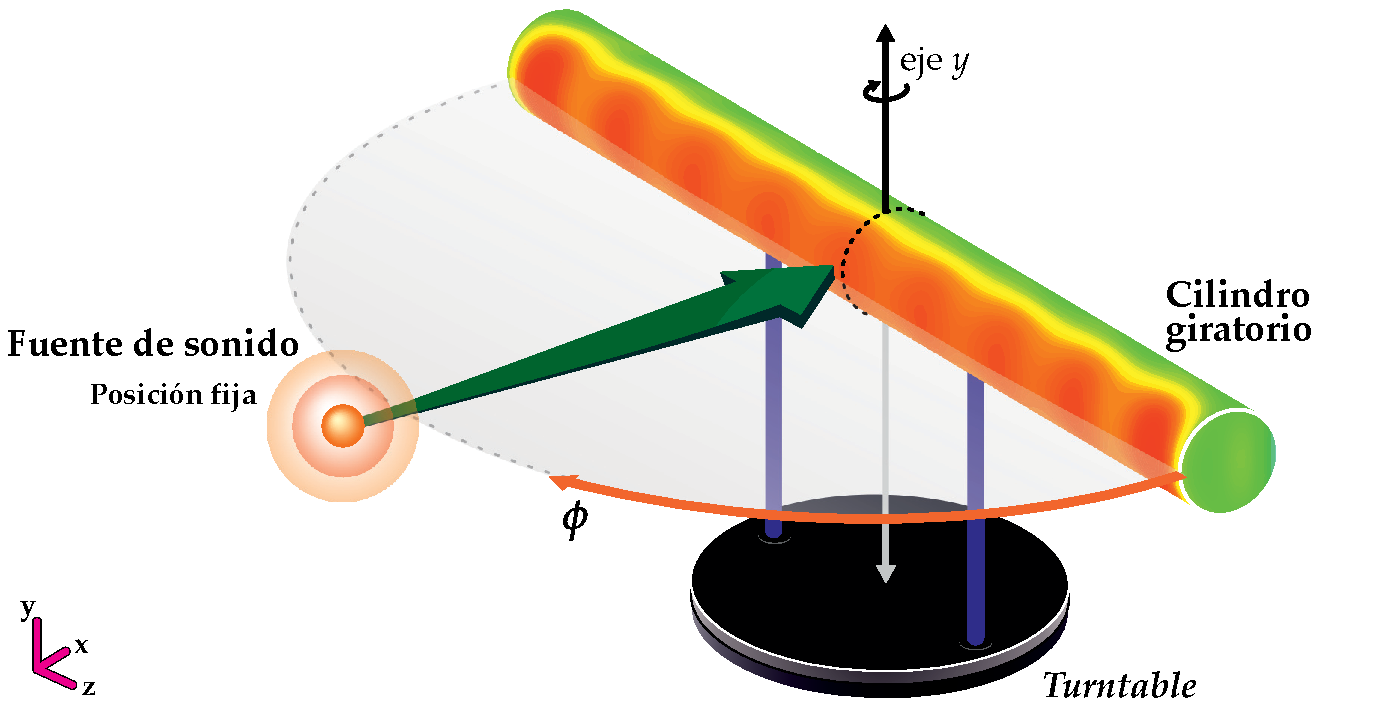
\includegraphics[width=0.74\linewidth]{figs/Measurement-Scheme-Fonseca-2013-sp.pdf}%
	\caption{Medición de \textit{beamforming} con arreglo cilíndrico (adaptado de Fonseca \cite{Fonseca-2013}).\\ Ejemplo de figura en dos columnas.}%
	\label{fig:beamforming}%
\end{figure*}

Serán adoptadas las unidades del Sistema Internacional (SI). Al escribir su trabajo en portugués o español, en los números, \textbf{use separador decimal coma} (conforme a reglas de la lengua portuguesa y española vigente), tanto sea en el texto como en tablas, figuras y/o gráficos, además de buscar siempre el uso de una misma precisión decimal al comparar números, por ejemplo: 3,0 es diferente de 3,00, aunque tenga la misma precisión decimal de 6,0.
En el caso de que el trabajo sea escrito en inglés, queda a criterio del autor utilizar punto o coma como separador decimal (siempre y cuando no se mezclen las notaciones).

Al escribir un número con su unidad\footnote{Las unidades son siempre escritas ``sin inclinación'', por ejemplo, 30~N/m$^2$.}, mantenga siempre el número junto a la unidad correspondiente, sin que exista quiebre de línea entre ellos (en Ms~Word utilice Ctrl + Shift + Espacio [o Alt + 0160], en \LaTeX\xspace coloque un ($\sim$) entre el número y la unidad). Por ejemplo, 3~m de distancia separa la entrada y la salida; 4.512,28~cm es la distancia medida.

Las ecuaciones deberán estar encajadas entre el texto (en Ms~Word utilice ``tabla'' simple) conforme el ejemplo de Ecuación~\eqref{eq:area-circ}. También deberán estar centradas y enumeradas secuencialmente, con la numeración ubicada en el lado derecho y entre paréntesis (ver ejemplo). Recuerde que las ecuaciones no son elementos textuales, deben ser puntuadas y el texto que les prosiga normalmente no es iniciado con letra mayúscula. Se recomienda colocar la nomenclatura inmediatamente después de haber presentado la variable en una ecuación.

El área del círculo (en m$^2$) es definida como
%
\begin{equation}
	A = \pi \, r^2\;,
\label{eq:area-circ}
\end{equation}
%
donde $r$ es el radio en metros (m). Recuerde que variables (como $r$ en este ejemplo) son escritas en \textit{cursiva} (tanto en la ecuación como en el texto). 

Sin embargo, \textbf{unidades, funciones y operadores matemáticos son escritos ``sin inclinación''} (sin aplicar cursiva). Por ejemplo, 32,0~N/m$^2$ fue la presión aplicada, o también
%
\begin{equation}
	\int_a^b p(\phi)\, \dt p\,
\label{eq:int}
\end{equation}
%
fue la integral calculada (observe que el operador diferencial ``$\tx{d}$''  está sin formato cursiva), para cada ángulo $\phi$ en grados. Como ejemplo de funciones se puede citar el seno, $\sen(\theta)$, o también $\log(y)$.

Texto en superíndice o subíndice solamente será en cursiva si fuese correspondiente a alguna variable pertinente. Case sea un ``nombre complementario'', la variable debe ser colocada sin inclinación, por ejemplo, $P\txu{total}$ corresponde a la presión total en Pa, o también $S\txup{\,tri}$ correspondiendo al área del triángulo en cm$^2$. Tratándose de una variable, por ejemplo, $i$, se debe escribir; la sumatoria fue calculada considerando $P_i$ hasta la $i$-ésima presión final correspondiente a 256.

En el caso de que se utilice texto, siglas o unidades en ecuaciones, su representación debe ser escrita sin formato cursiva, por ejemplo:
%
\begin{equation}
	\text{densidad} = \frac{\tx{masa}}{\;\;\tx{volumen}\;\;}\,,
\label{eq:densidad}
\end{equation}

donde en el SI (Sistema Internacional de Unidades) la unidad de densidad es en kilogramos por metro cúbico (kg/m$^3$).
%
En el caso de que fuese necesario citar en el texto una ecuación que ya fue presentada, se debe proceder de la siguiente manera: Ecuación~\eqref{eq:densidad} --- con solamente la primera letra en mayúscula y con el número correspondiente entre paréntesis.

%%%%%%%%%%%%%%%%%%%%%%%%%%%%%%%%%%%%%%%%%%%%%%%%%%%%%%%%%%%%%%%%%%%%%%%%%%%%%%%%%%%%%%%%%%%%%%%%%%%%%%%%%%%%%%%%%%%
\subsection{Figuras, tablas, cuadros y códigos}

Las figuras y tablas deben tener lugar en el texto, con preferencia, inmediatamente después de los párrafos a los cuales se refieren. Antes de presentar una figura, tabla y códigos sería conveniente realizar una mención durante el texto que los precede para una mejor orientación del lector. Las figuras, tablas y cuadros deben contener todos los elementos de formato y contenido con el fin de que sean interpretados correctamente, sin necesidad de recurrir al texto precedente para buscar informaciones adicionales. Se debe separar del texto, las tablas y figuras con \textbf{una (1) línea} en blanco antes y después (12~pt).

% En Latex esto ya está configurado automáticamente.

\begin{table*}[!b]
  \centering \ratb{1.3} 
  \caption{Propiedades microgeométricas y macroscópicas de las capas porosas CPA~1 e CAUQ-B\\ (adaptado de Mareze \etal \cite{Mareze-2017}). Ejemplo de tabla de dos columnas.}
	\fontsize{11}{12}\selectfont 
    \begin{tabular}{C{2.9cm} | C{1.5cm} | C{1.5cm} | C{1.5cm} | C{1.5cm} | C{1.5cm} | C{1.0cm}| C{1.0cm}}
    \toprule
		\SetRowColor{LightOrange}
    \textbf{ Muestra / Parámetro } & $L\txu{p}$ \qquad [$\upmu$\! m] & $L\txu{a}$ \qquad [$\upmu$\! m] & $D\txu{p}$ \qquad [$\upmu$\! m] & $D\txu{a}$ \qquad [$\upmu$\! m] & $\sigma$ [Ns/m\txup{4}] & {$\phi$\quad [--]} & $\alpha_{\infty}$ [--]\\
	  \midrule
		CPA 1 $\Rightarrow$  3,0\% &	1359,81 & 1492,51 & 2344,05 & 1425,67 &	5131 &	0,218 &	1,63\\
		\rowcolor[gray]{.95} CAUQ-B $\Rightarrow$ 4,5\%	& 1598,29 &	701,24 & 2126,46 & 895,34 &	54989 &	0,070 &	2,89\\
    \bottomrule
    \end{tabular}
    \label{tab.exemplo}%
\end{table*}%

Las figuras, tablas y cuadros deberán estar centrados y numerados secuencialmente (ver ejemplo en las Figuras~\ref{fig:beamforming}, \ref{subfig.exemplo} y \ref{fig:C80}; Tabla~\ref{tab.exemplo}; Cuadro~\ref{quad.exemplo} y Código~\ref{code.matlalatex}). Estos podrán ser colocados en una o dos columnas dependiendo de su contenido. En el caso de dos columnas, se recomienda posicionar el objeto en la parte superior o inferior de las páginas. Intente utilizar figuras y gráficos en los cuales su contenido pueda ser completamente comprendido. 

El rótulo y número de las figuras, seguido de la leyenda, debe aparecer inmediatamente abajo de la figura y centrado (10~pt). Caso utilice figuras de otros autores (o fuentes), adaptados o no, indique la fuente inmediatamente después de la leyenda descriptiva. Ver ejemplo de la Figura~\ref{fig:beamforming}.

El rótulo, número y leyenda de las tablas (cuadros y códigos también) deben aparecer centrados en la parte superior (ver Tabla~\ref{tab.exemplo}). La fuente (cuando sea necesario) de la tablas debe ser presentada de acuerdo con la publicación original. La Tabla~\ref{tab.exemplo} presenta un ejemplo del estilo a ser utilizados (el contenido de la tabla podrá contener tipografía menor que la del texto). Además, se recomienda que el sistema de referencias cruzadas sea automático. Recuerde que todos los objetos, como figuras y tablas, deben ser citados en el texto.


\begin{figure}[H]
  %\ContinuedFloat %% para continuar a partir da figura anterior
  \centering
	\subfloat[Figura A.]{\label{fig.figA}
\includegraphics[height=23mm,page=2]{FIA-logo.pdf}}
	\qquad
  \subfloat[Figura B.]{\label{fig.figB}
\includegraphics[height=23mm,page=2]{FIA-logo.pdf}}	
  \caption{Ejemplo de figuras lado a lado.}
  \label{subfig.exemplo}
\end{figure}

\begin{figure}[ht!]
	\centering \vspace{-3mm}
        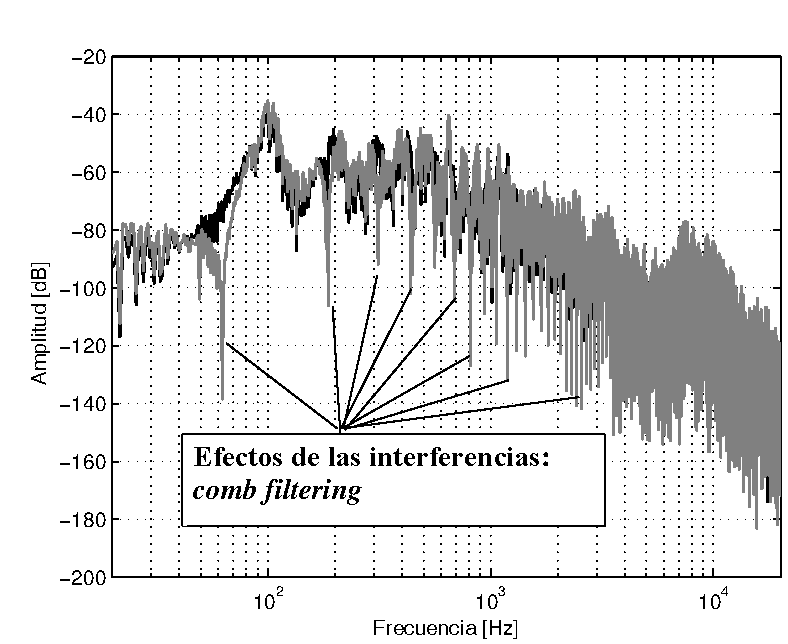
\includegraphics[width=0.98\linewidth,page=1]{figs/Combfilter-Brandao-2017-sp.pdf}
        \vspace{-0.4em}
        \caption{$C_{80}$ para salas distintas. Las figuras pueden ser colocadas lado a lado (adaptado de Brandão \cite{Brandao-2017}).}
	\label{fig:C80}%
\end{figure}


\begin{quadro}[ht!]
%\vspace{-2mm}
  \centering \ratb{1.3} \setlength\aboverulesep{0pt} \setlength\belowrulesep{0pt}
  \caption{Este es un ejemplo de un cuadro.}
	\fontsize{11}{12}\selectfont 
    \begin{tabular}{| C{2.8cm} | C{1.8cm} | C{1.8cm} |}
    \hline
	\SetRowColor{LightBlue}
    \textbf{ Experimento / Tipo } & \textbf{Exp. 1} & \textbf{Exp. 2}\\
	\midrule
		Tipo 1& Verde & Amarilla\\
		\rowcolor[gray]{.95} Tipo 2 & Azul & Blanco\\
    %\bottomrule
		\hline
    \end{tabular}
    \label{quad.exemplo}%
% 	\vspace{-4mm}
\end{quadro}%


%% Modelo de figuras lado a lado usando minipage
%\begin{figure*}[b]
    %\centering
    %\begin{minipage}[t]{.48\textwidth}
        %\centering
        %
\includegraphics[width=1\linewidth,page=2]{FIA-logo.pdf}
        %\caption{Figura do lado esquerdo.}
        %\label{fig:ladoE}
    %\end{minipage}%
		%\quad
    %\begin{minipage}[t]{0.48\textwidth}
        %\centering
        %
\includegraphics[width=1\linewidth,page=2]{FIA-logo.pdf}
        %\caption{Figura do lado direito.}
        %\label{fig:ladoD}
    %\end{minipage}
%\end{figure*}

Se recomienda que los gráficos, figuras, fotos y cualquier archivo gráfico, sean colocados en el texto en formato \!\texttt{.jpg} y/o \texttt{.png} con buena calidad (o también en formato vectorial en \texttt{.pdf} para usuarios do \LaTeX\xspace). Asegúrese que los elementos gráficos y figuras sean legibles (sobre todo si la información que contienen es relevante).

La distribución de este \textit{template} de \LaTeX\xspace incluye el paquete \ttc{Codes2Latex.sty}\footnote{El paquete aún está en desarrollo (sin documentación detallada). Para más detalles, consulte el archivo \ttc{sty}.}, que permite la posibilidad de documentar códigos genéricos y en lenguaje Matlab, Fortran, Python, LabView y Latex de forma organizada (observe el Código~\ref{code.matlalatex}).

\begin{matlabcode}[Haciendo que Matlab escriba Latex.]{code.matlalatex}
  syms x
  f = taylor(log(1+x));
  latex(f)
\end{matlabcode}

Todos los elementos (figuras y gráficos, por ejemplo) pueden ser coloridos o en tonos de gris. Evite utilizar elementos textuales de otros autores sin citarlos o sin autorización. Es esencial que las figuras que se presenten en el texto estén en el mismo idioma que el del artículo. No se aceptarán citaciones indirectas como \textit{Google Imágenes}, por ejemplo, así como también se recomienda evitar el abuso de bases de conocimiento volátiles.

Las referencias cruzadas deben ser posibles de realizar en todos los objetos presentes en el texto, por ejemplo: Figura~\ref{fig:beamforming} y Tabla~\ref{tab.exemplo} (apenas con la primera letra mayúscula). Además, el número de la figura o de la tabla no debe estar separado de la palabra Figura o Tabla en la siguiente línea. Para evitarlo, en Ms Word, use Ctrl + Shift + Espacio, y en \LaTeX, inserte una tilde ($\sim$) entre la palabra Figura y el comando \verb=\ref= o entre la palabra Tabla y el comando \verb=\ref=. Caso exista una subfigura, utilice Figura~\subref*{fig.figA}, por ejemplo.


%%%%%%%%%%%%%%%%%%%%%%%%%%%%%%%%%%%%%%%%%%%%%%%%%%%%%%%%%%%%%%%%%%%%%%%%%%%%%%%%%%%%%%%%%%%%%%%%%%%%%%%%%%%%%%%%%%%
\section{Tipos de artículo}

El evento aceptará \textbf{envíos originales} (es decir, aún no publicados) de investigaciones científicas y aplicaciones de ingeniería, arquitectura, audio, física, matemática, fonoaudiología y áreas y subáreas relacionadas. De esta forma, serán considerados los siguientes tipos de documentos:
%
\begin{itemize}[noitemsep,topsep=2ex] \itemsep=12pt
	\item \textbf{Artículos técnicos y aplicados} (\textit{Technical and applied papers}): presentan material original a partir de aplicaciones de técnicas conocidas y/o en desarrollo. Debe presentar métodos aplicados que estén de acuerdo con normativas y/o que presenten resultados pertinentes. Es esencial que sean de interés de investigadores y profesionales del tema propuesto.
	
	\item \textbf{Artículos científicos} (\textit{Scientific papers}): 
	contienen material original (ideas, modelos, experimentos, \etc) no publicados, que contribuyen substancialmente para el avance de la ciencia en aquel tema. El artículo debe establecer una relación entre su contenido y el \textit{estado del arte} ya publicado.

	\item \textbf{Artículos de revisión} (\textit{Review papers}):
	discuten el \textit{estado del arte} sobre el tema elegido, aclarando desde aspectos básicos hasta los sofisticados. Este tipo de envío debe ser completo en lo que respecta a la literatura, cubriendo en buena parte las ideas, modelos, experimentos, \etc ya desarrollados, aunque no concuerden con la opinión del autor. Es importante que el tema sea de interés para la comunidad científica.
\end{itemize}

\vspace{5pt}

Las áreas temáticas del evento incluyen:
%	
\begin{itemize}[noitemsep,topsep=-1ex] \itemsep=1.0pt
\item[\textbullet] Acústica Ambiental;
\item[\textbullet] Acústica de Edificaciones;
\item[\textbullet] Acústica de la Audición y del Habla;
\item[\textbullet] Acústica de Salas;
\item[\textbullet] Acústica Musical;
\item[\textbullet] Acústica Submarina;
\item[\textbullet] Acústica Vehicular;
\item[\textbullet] Acústica Virtual;
\item[\textbullet] Acústica General;
\item[\textbullet] Aeroacústica;
\item[\textbullet] Audio e Electroacústica;
\item[\textbullet] Bioacústica;
\item[\textbullet] Control de Ruido;
\item[\textbullet] Educación en Acústica;
\item[\textbullet] INAD e IYS~2020+;
\item[\textbullet] Legislaciones y normalización en Acústica;
\item[\textbullet] Materiales acústicos;
\item[\textbullet] Mediciones en Acústica y Vibraciones;
\item[\textbullet] Métodos Numéricos en Acústica y Vibraciones;
\item[\textbullet] Paisaje sonoro;
\item[\textbullet] Procesamiento de Señales;
\item[\textbullet] Psicoacústica;
\item[\textbullet] Ruido y Vibraciones en ambiente laboral;
\item[\textbullet] Técnicas de imagen acústica;
\item[\textbullet] Ultrasonido; y
\item[\textbullet] Vibraciones y Vibroacústica.
\end{itemize}
	

%%%%%%%%%%%%%%%%%%%%%%%%%%%%%%%%%%%%%%%%%%%%%%%%%%%%%%%%%%%%%%%%%%%%%%%%%%%%%%%%%%%%%%%%%%%%%%%%%%%%%%%%%%%%%%%%%%%
%%%%%%%%%%%%%%%%%%%%%%%%%%%%%%%%%%%%%%%%%%%%%%%%%%%%%%%%%%%%%%%%%%%%%%%%%%%%%%%%%%%%%%%%%%%%%%%%%%%%%%%%%%%%%%%%%%%
\section{Organización del trabajo}

La estructura del artículo deberá contemplar al menos los siguientes ítems:
%
\begin{itemize}[noitemsep,topsep=-1ex] \itemsep=3pt
	\item Introducción: visión general sobre el asunto con definición de los objetivos del trabajo, indicando su relevancia.
	\item Fundamentos: fundamentalmente en artículos científicos, la fundamentación teórica principal necesaria para el entendimiento del texto debe ser presentada y referenciada;
	\item Desarrollo: cómo el trabajo fue realizado, incluyendo detalles de la teoría, materiales y métodos utilizados;
	\item Resultados y discusiones: parciales o concluyentes, conforme a la modalidad de trabajo, haciendo referencia a las mediciones y cálculos estadísticos aplicados, se fuese el caso;
	\item Conclusiones o consideraciones finales: tomar como base las discusiones y objetivos, presentando consideraciones que concluyan el estudio/aplicación realizado;
	\item Agradecimientos: opcional, cuando fuese pertinente; y
	\item Referencias: presentar la bibliografía citada en el texto.
\end{itemize}
%
No es necesario que existan secciones con estos nombres. La organización del trabajo depende del tipo artículo.
Otros elementos postextuales como apéndices son opcionales, desde que estos (en el total), no excedan el límite total de 12 páginas.

%%%%%%%%%%%%%%%%%%%%%%%%%%%%%%%%%%%%%%%%%%%%%%%%%%%%%%%%%%%%%%%%%%%%%%%%%%%%%%%%%%%%%%%%%%%%%%%%%%%%%%%%%%%%%%%%%%%
\subsection{Citaciones y referencias}

Para construir las referencias se debe utilizar la norma vigente. Las referencias deben ser \textbf{enumeradas conforme el orden de aparición}, utilizando corchetes \cite{Gomes-2015}. Todas las referencias deben estar citadas en el texto. Las referencias \cite{Mareze-2017,Fonseca-2013,Brandao-2017,Gomes-2015,Oppenheim-2010,Muller-2001,Mareze-2019,Borges-2018,Ristow-2016} de este modelo de artículo son apenas ilustrativas (a efecto de comprensión).

% En Latex, se recomeinda usar unsrtnat y unsrtnat-br.

La sección de referencias debe ser colocada al final del documento.  Cada una de las entradas de esta sección debe ser escritas en tipografía con tamaño 10~pt, espaciamiento simple y espaciamiento de párrafo de 6~pt. Este \textit{template} de \LaTeX\xspace utiliza el paquete {\ttfamily natbib} para la organización de las referencias. Además, se recomienda la utilización de gestores de banco de datos de bibliografía como \href{http://www.jabref.org/}{JabRef}, \href{http://www.mendeley.com}{Mendeley} y \href{https://www.zotero.org/}{Zotero}. En especial, para usuarios de Ms~Word, Mendeley tiene un \textit{plugin} para dar formato e ingresar las referencias en el documento .docx.

Dependiendo del contexto, el nombre del autor puede o no ser escrito, conforme a los siguientes ejemplos:
%
\begin{itemize}[noitemsep,topsep=0ex] \itemsep=4pt
	\item 	``... Mareze \etal \cite{Mareze-2019} trabajaron con absorción de materiales porosos...'', o
	\item ``... para el estudio de acústica de salas \cite{Brandao-2017} se recomienda la lectura de un libro texto...'', o
	\item ``... aplicando la Transformada de Fourier en las señales de entrada \cite{Oppenheim-2010}. '', o también
	\item ``... Fonseca (2013) demostró el cálculo de difracción para superficies cilíndricas~\cite{Fonseca-2013}.''
\end{itemize}
%
Todos los autores que están presentes en las referencias deben estar citados en el texto.

En las referencias con hasta tres autores, por ejemplo, Müller e Massarani \cite{Muller-2001}, ambos deben ser citados (cuando son mencionados). En el caso de más de tres autores, por ejemplo,  Gomes \etal \cite{Gomes-2015} se debe citar solamente el último apellido del primer autor seguido de la expresión ``\etal''. También, al citar más de una referencia, utilice solamente un corchete. Vea los siguientes ejemplos:
%
\begin{itemize}[noitemsep,topsep=0ex] \itemsep=8pt
	\item ``Trabajos en temas de acústica e vibraciones \cite{Mareze-2017,Fonseca-2013,Brandao-2017}.''
	\item ``Trabajos en temas de acústica \cite{Mareze-2017,Oppenheim-2010,Muller-2001,Mareze-2019}.''
	\item ``Trabajos con análisis estadístico \cite{Mareze-2017, Brandao-2017, Borges-2018}.''
		\item \textbf{No usar este estilo:} ``Trabajos con análisis estadístico \cite{Mareze-2017}, \cite{Brandao-2017}, \cite{Ristow-2016}.''
\end{itemize}
%
Se recomienda que las referencias sean ordenadas y compactadas (con guión medio) como en \cite{Mareze-2017,Oppenheim-2010,Muller-2001,Mareze-2019}.

En la sección de referencias, siempre que sea posible, incluya el ISBN, ISSN, DOI\footnote{Para usuarios de Latex basta usar el campo ``doi'' del correspondiente repositorio \texttt{.bib}.} (con link) y/o link con la dirección online en la que el documento citado se encuentra disponible.

%%%%%%%%%%%%%%%%%%%%%%%%%%%%%%%%%%%%%%%%%%%%%%%%%%%%%%%%%%%%%%%%%%%%%%%%%%%%%%%%%%%%%%%%%%%%%%%%%%%%%%%%%%%%%%%%%%%
\section{Envío del documento y\\ evaluación}

Después de la aprobación de los resúmenes enviados en el sitio web del evento \url{www.fia2020.com.br}, los autores serán convocados para elaborar los trabajos completos. Detalles acerca del registro pueden ser consultados también en el sitio web del evento o con la comisión organizadora.

Es responsabilidad de los autores la preparación del envío de los artículos en su formato final. Por este motivo, se pide que sean verificados con atención el formato de sus artículos, especialmente gráficos y fotos, en relación a su legibilidad y calidad digital (y para impresión). \textbf{Los artículos deberán ser enviados en formato PDF (con tamaño máximo de 10~Mb)}.

Los metadatos del PDF para usuarios de \LaTeX\xspace son generados automáticamente, usuarios de Ms~Word deben corroborarlos al momento de la conversión.

% El uso de PDF-a es opcional.
Investigaciones que incluyan personas (o seres vivos , en general), como en acústica subjetiva o fisiológica, por ejemplo, deben aclarar en el artículo el término de aprobación del Comité de Ética, caso sea pertinente.

%%%%%%%%%%%%%%%%%%%%%%%%%%%%%%%%%%%%%%%%%%%%%%%%%%%%%%%%%%%%%%%%%%%%%%%%%%%%%%%%%%%%%%%%%%%%%%%%%%%%%%%%%%%%%%%%%%%
\section{Modelos para Word y \LaTeX}

El modelo de \LaTeX\xspace (\texttt{.tex}) fue escrito en codificación UTF8, con el objetivo que sea compatible con Windows, Mac, Linux y \href{https://www.overleaf.com/read/rnfjxkknksnd}{Overleaf}\footnote{\url{https://www.overleaf.com/read/rnfjxkknksnd}.}. Puede ser utilizado libremente para la elaboración de los artículos.

El modelo de \texttt{.docx} fue generado en Microsoft Word 2016 y, con esto, sus funcionalidades de espaciamiento y configuraciones están garantizadas para esa versión.

El autor de este texto y de los modelos es el profesor William D'Andrea Fonseca, de Ingeniería Acústica (EAC) de la Universidad Federal de Santa Maria (UFSM).
%
La revisión fue realizada por el profesor Stephan Paul (UFSC).
El modelo de Ms~Word fue finalizado por el estudiante Felipe Ramos de Mello (EAC/UFSM).

La versión en español fue traducida por Diego Martin Tuozzo y revisada por William D'Andrea Fonseca.
%
La traducción al inglés fue realizada por Thiago Morphy y los profesores Stephan Paul (UFSC) y William D'Andrea Fonseca (UFSM) --- la corrección de pruebas corrió a cargo de Joseph Lacey. 

Todas estas versiones están disponibles con links en el \href{http://fia2020.com.br}{sitio web del evento}, en \href{https://www.overleaf.com/read/rszcxtwshzfr}{Overleaf} (\href{https://www.overleaf.com/read/rnfjxkknksnd}{PT-BR}, \href{https://www.overleaf.com/read/rszcxtwshzfr}{SP} y \href{https://www.overleaf.com/read/hgryywpgmxdx}{EN}) y en \href{https://github.com/willdfonseca/fia2020}{GitHub}\footnote{\url{https://github.com/willdfonseca/fia2020}.}.

%%%%%%%%%%%%%%%%%%%%%%%%%%%%%%%%%%%%%%%%%%%%%%%%%%%%%%%%%%%%%%%%%%%%%%%%%%%%%%%%%%%%%%%%%%%%%%%%%%%%%%%%%%%%%%%%%%%
\section{Consideraciones finales}

Lo que se pretende con este \textit{artículo modelo} es listar de forma organizada y aclarar las instrucciones para el envío de artículos para el FIA 2020 integrando el XIX Encuentro de la Sobrac. Este documento puede ser utilizado como modelo solamente cambiando el contenido.

%%%%%%%%%%%%%%%%%%%%%%%%%%%%%%%%%%%%%%%%%%%%%%%%%%%%%%%%%%%%%%%%%%%%%%%%%%%%%%%%%%%%%%%%%%%%%%%%%%%%%%%%%%%%%%%%%%%
\section{Agradecimientos}

Se fuese pertinente, realice los agradecimientos.
%
En caso de trabajos con auxilio o estímulo financiero, utilice esta sección para brindar detalles.

En el caso de este documento, el comité organizador quiere agradecer a todos su colaboración con el evento.
%%%%%%%%%%%%%%%%%%%%%%%%%%%%%%%%%%%%%%%%%%%%%%%%%%%%%%%%%%%%%%%%%%%%%%%%%%%%%%%%%%%%%%%%%%%%%%%%%%%%%%%%%%%%%%%%%%%%
%%%%%%%%%%%%%%%%%%%%%%%%%%%%%%%%%%%%%%%%%%%%%%%%%%%%%%%%%%%%%%%%%%%%%%%%%%%%%%%%%%%%%%%%%%%%%%%%%%%%%%%%%%%%%%%%%%%%
%%% Referências
\renewcommand{\refname}{Referencias} 
% \bibliographystyle{unsrtnat} 
\bibliographystyle{unsrtnat-br}  % Estilo semelhante ao padrão brasileiro
{{\fontrefs \bibliography{bibliografia}}
%%%%%%%%%%%%%%%%%%%%%%%%%%%%%%%%%%%%%%%%%%%%%%%%%%%%%%%%%%%%%%%%%%%%%%%%%%%%%%%%%%%%%%%%%%%%%%%%%%%%%%%%%%%%%%%%%%%
%%%%%%%%%%%%%%%%%%%%%%%%%%%%%%%%%%%%%%%%%%%%%%%%%%%%%%%%%%%%%%%%%%%%%%%%%%%%%%%%%%%%%%%%%%%%%%%%%%%%%%%%%%%%%%%%%%%
\appendix
\section{Ejemplo de apéndice}

Este es un ejemplo de apéndice, generalmente se colocan informaciones adicionales o deducciones producidas por los autores.
Este modelo (\textit{template} de \LaTeX) tiene algunos comandos adicionales que facilitan la escritura, como, por ejemplo,  \F\xspace para simbolizar la Transformada de Fourier. Para conocer mejor los comandos, consulte el archivo  \texttt{FIA2020.sty}.

}
%%%%%%%%%%%%%%%%%%%%%%%%%%%%%%%%%%%%%%%%%%%%%%%%%%%%%%%%%%%%%%%%%%%%%%%%%%%%%%%%%%%%%%%%%%%%%%%%%%%%%%%%%%%%%%%%%%%
%%%%%%%%%%%%%%%%%%%%%%%%%%%%%%%%%%%%%%%%%%%%%%%%%%%%%%%%%%%%%%%%%%%%%%%%%%%%%%%%%%%%%%%%%%%%%%%%%%%%%%%%%%%%%%%%%%%
% Exemplo de códigos em duas colunas
%\onecolumn
%\section{Escrevendo um código de apêndice em uma coluna}
%
% Caso existam códigos muito extensos, o apêndice pode ser convertido para uma coluna, como exemplificado nesta seção com o Código~\ref{code.fc}.
%
%\inputcodeLatin{Matlab}{Exemplo de inclusão de código (de Matlab) em duas colunas.}{code.fc}{FC.m}

%%%%%%%%%%%%%%%%%%%%%%%%%%%%%%%%%%%%%%%%%%%%%%%%%%%%%%%%%%%%%%%%%%%%%%%%%%%%%%%%%%%%%%%%%%%%%%%%%%%%%%%%%%%%%%%%%%%
% \clearpage  \listoftodos % This temporary list may help the writing of the paper.
%%%%%%%%%%%%%%%%%%%%%%%%%%%%%%%%%%%%%%%%%%%%%%%%%%%%%%%%%%%%%%%%%%%%%%%%%%%%%%%%%%%%%%%%%%%%%%%%%%%%%%%%%%%%%%%%%%%
%%%%%%%%%%%%%%%%%%%%%%%%%%%%%%%%%%%%%%%%%%%%%%%%%%%%%%%%%%%%%%%%%%%%%%%%%%%%%%%%%%%%%%%%%%%%%%%%%%%%%%%%%%%%%%%%%%%
\end{document}
%%%%%%%%%%%%%%%%%%%%%%%%%%%%%%%%%%%%%%%%%%%%%%%%%%%%%%%%%%%%%%%%%%%%%%%%%%%%%%%%%%%%%%%%%%%%%%%%%%%%%%%%%%%%%%%%%%%
% EOF